\chapter{LaTeX Docker}
\ChapterLabel{LatexDocker}
\index{LaTeX!Docker}
\index{TeX Live}
\index{Overleaf}

\section{Overview}
Overleaf compiles every project with \gls{texlive}, run inside containers on
its servers. This chapter reproduces that setup locally: a Docker image built on
the official \texttt{texlive/texlive} image compiles a simple LaTeX document
from a folder on the host. The same container builds this group document, so
every member gets an identical toolchain without installing MacTeX or MiKTeX,
and the build can later run unchanged in a CI pipeline.

\section{How It Works}
\begin{enumerate}
\item The image contains a full TeX Live installation plus \texttt{latexmk},
which reruns \texttt{pdflatex}, BibTeX, and index tools until cross-references
settle.
\item At run time the current host folder is bind-mounted at
\texttt{/workdir}, so the container reads the \texttt{.tex} source and writes
the PDF back to the host.
\item The container is started with \texttt{--rm}, so it is deleted after each
compile. Only the image persists.
\end{enumerate}

\section{Project Files}
\begin{minted}{text}
latex-docker/
  Dockerfile    image definition
  hello.tex     simple test document
  build.sh      builds the image and compiles a .tex file
  .gitignore    keeps auxiliary files out of Git
\end{minted}

\noindent\textbf{Dockerfile} --- \texttt{ENTRYPOINT} fixes the compiler and
flags, while \texttt{CMD} supplies a default file name that can be overridden on
the \texttt{docker run} line. \texttt{-shell-escape} is required by
\texttt{minted}; it lets LaTeX call the Pygments highlighter, so it should only
be used on trusted documents.
\inputminted{docker}{../latex-docker/Dockerfile}

\medskip\noindent\textbf{hello.tex} --- a small document that exercises text,
math, and a \texttt{minted} code block:
\inputminted{latex}{../latex-docker/hello.tex}

\medskip\noindent\textbf{build.sh} --- one command to build and compile:
\inputminted{bash}{../latex-docker/build.sh}

\section{Commands Run}
\subsection{Build the Image}
The base image is large (about 2.7\,GB compressed) because it contains the
complete TeX Live distribution, the same scheme Overleaf offers. It is pulled
once and then cached.
\begin{minted}{bash}
cd latex-docker
docker pull texlive/texlive:latest
docker build -t latex-builder .
\end{minted}
\inputminted{console}{../evidence/latex-docker-build.txt}

\subsection{Compile the Document}
\begin{minted}{bash}
docker run --rm -v "$PWD":/workdir latex-builder hello.tex
\end{minted}
The output below is abridged to \texttt{latexmk}'s run summary; the TeX Live
2026 \texttt{pdflatex} ran three times before reporting that the PDF was up to
date.
\inputminted{console}{../evidence/latex-docker-run.txt}
Figure~\ref{Figure:LatexDockerOutput} shows the resulting PDF.

\begin{figure}[htbp]
\centering
\setlength{\fboxsep}{0pt}\fbox{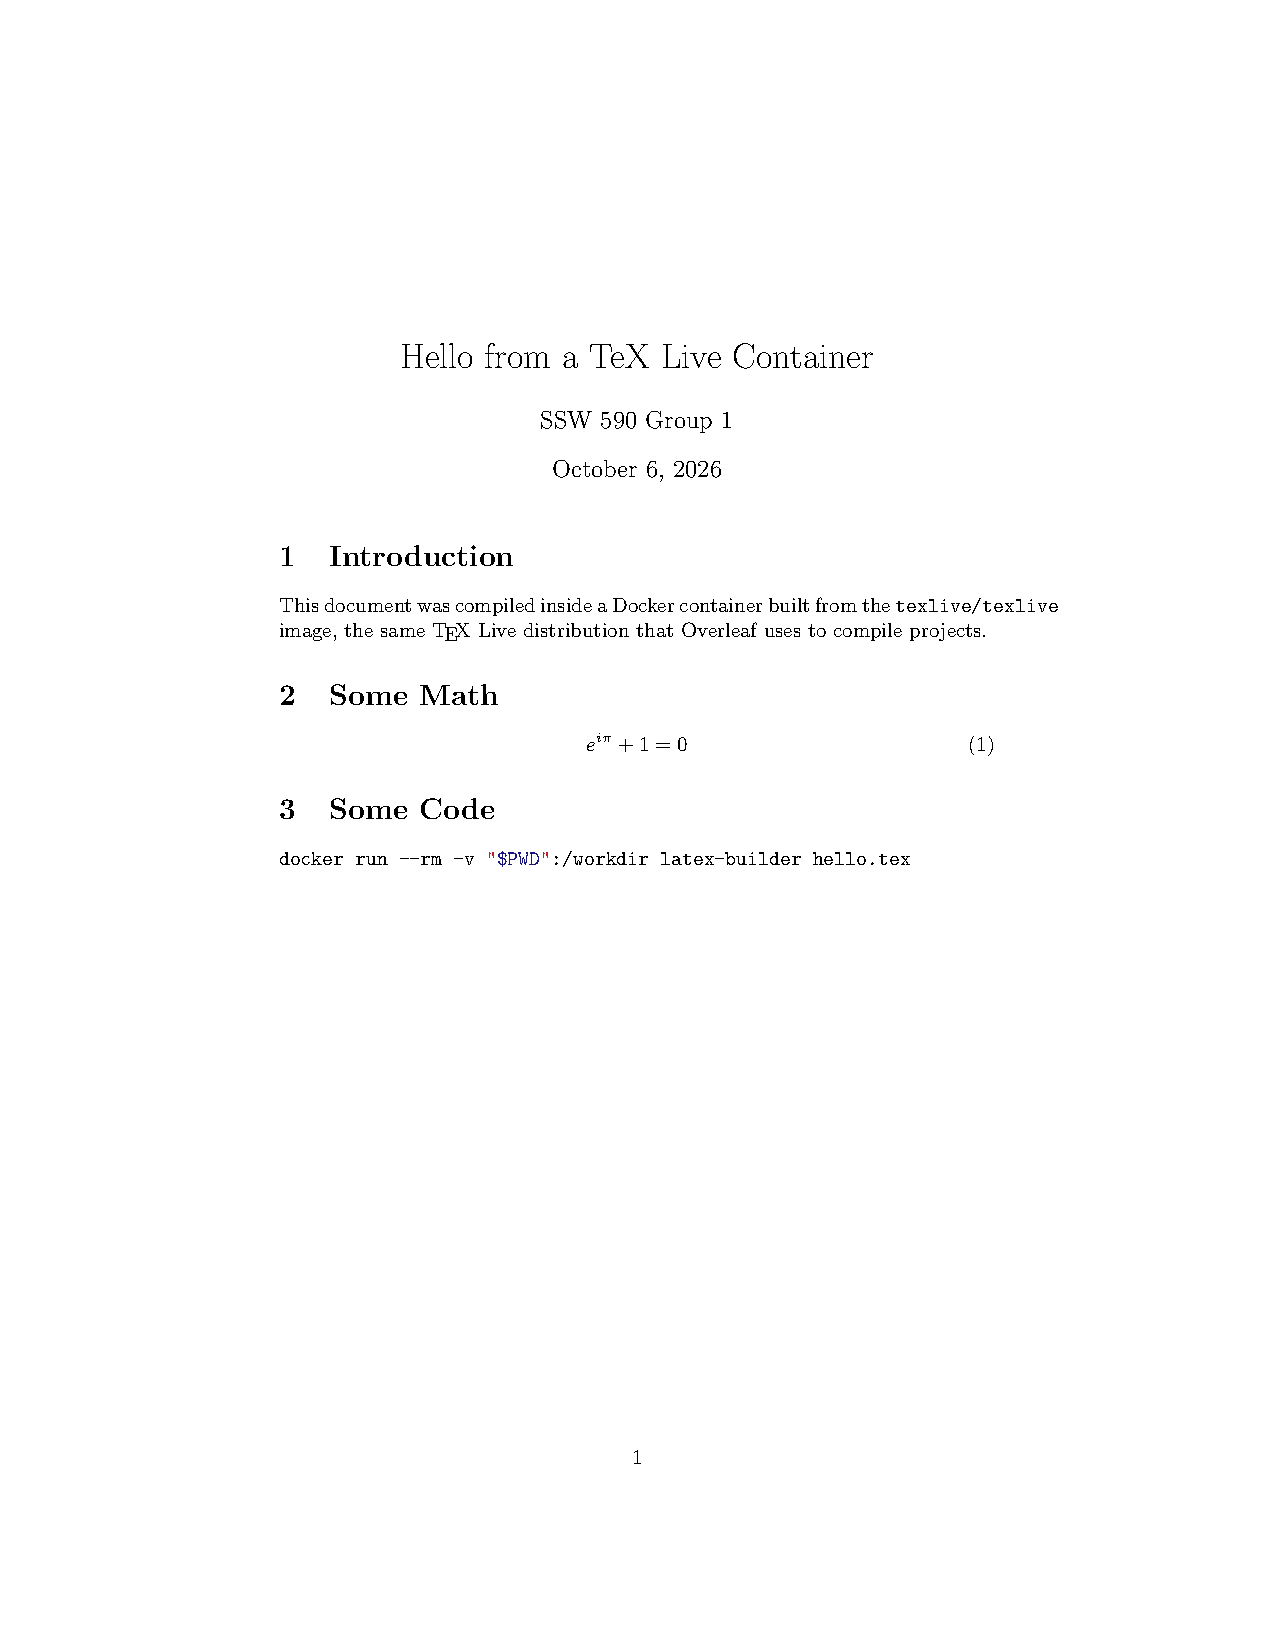
\includegraphics[width=0.75\linewidth,trim=90 420 90 90,clip]{../evidence/latex-docker-hello.pdf}}
\caption{Top of \texttt{hello.pdf} compiled by the \texttt{latex-builder} container.}
\label{Figure:LatexDockerOutput}
\end{figure}

\subsection{Compile This Group Document}
The same image builds this report. From the repository root, the whole
repository is mounted so the report can include source files from
\texttt{website/}, \texttt{deploy/}, and \texttt{evidence/}:
\begin{minted}{bash}
docker run --rm -v "$PWD":/workdir -w /workdir/report \
  latex-builder devopsAssignment.tex
\end{minted}

\section{Comparison with Overleaf}
\begin{tabularx}{\linewidth}{L{3.0cm}YY}
\caption{Overleaf Compared with the LaTeX Container\label{Table:OverleafVsDocker}}\\
\toprule \textbf{Aspect} & \textbf{Overleaf} & \textbf{LaTeX Docker}\\ \midrule
\endfirsthead
\toprule \textbf{Aspect} & \textbf{Overleaf} & \textbf{LaTeX Docker}\\ \midrule
\endhead \bottomrule \endlastfoot
Engine & TeX Live in server-side containers & TeX Live in a local container\\
Collaboration & Real-time editing and comments & Git branches and pull requests\\
Version control & Built-in history; Git sync on paid plans & Native Git in the group repo\\
Compile limits & Timeout on free plan & Limited only by the machine\\
Offline use & No & Yes, once the image is pulled\\
Automation & Manual recompile & Scriptable; reusable in CI (\ChapterRef{ProjectProposal})\\
\end{tabularx}

\section{Troubleshooting}
\begin{itemize}
\item \textbf{Apple silicon.} \texttt{texlive/texlive} publishes
\texttt{arm64} images, so it runs natively on Apple silicon Macs without
emulation.
\item \textbf{File not found.} The \texttt{.tex} file must be inside the
mounted folder; paths are resolved relative to \texttt{/workdir}.
\item \textbf{Glossaries.} \texttt{latexmk} does not run
\texttt{makeglossaries} by default; \texttt{report/latexmkrc} adds that rule
for this document.
\end{itemize}
